% Project Proposal Document
\documentclass[review]{cmpreport}
\makeatletter
\input{t1pcr.fd}
\makeatother
\setlength{\footnotesep}{3ex}
\title{\Codex: A Website and Progressive Web App in Node.js \& React for table-top role-playing games \\ Living Report}
\author{Christopher Alastair Irvine}
\registration{100036248}
\supervisor{Dr Katharina Huber}
\ccode{CMP-6013Y}
\summary{This document is the Living Report for Codex}
\acknowledgements{
	I would like to thank Dr Katharina Huber for taking on the supervision of this project, 
	and guiding me towards greatness. Additionally I would like to thank Wizards of the Coast 
	for their generosity and kindness in allowing the use of their Intellectual Property for this project.
}
\usepackage{rotating}
\newcommand{\ueacmp}{UEA School of Computing Sciences}
\newcommand{\WotC}{Wizards of the Coast}
\newcommand{\dnd}{D\&D}
\newcommand{\sem}{Software Engineering Model}
\newcommand{\sems}{Software Engineering Models}
\newcommand{\Codex}{\textsc{Codex}}
\newcommand{\AgileSolo}{\emph{Agile Solo}}
% EOF Preamble and Macros
	
% BOF Document
\begin{document}
	% BOF Introduction
	\section{Introduction} \label{intro}
	% Introduce Dungeons and Dragons, when it was created and how the DM has remained at the center of the game.	
	Over the years, \emph{Dungeons and Dragons} (\dnd) have entertained millions of players across the world (\cite{DnDOriginal}). Throughout the various editions of this popular table-top role-playing game, the \emph{Dungeon Master} (DM) has formed the core of every group. The role of a DM is to provide content for the players (party) to explore in addition to acting as a; referee, ally, enemy, narrator, historian, peace-keeper and above all friend (\cite{DnDPeople}, \cite{DungeonMaster}). 
	
	The average \dnd \ campaign occurs once a week, for four hours, until the campaign is finished. Typically, a DM will spend between 5 and 15 hours preparing content per week, but the work of a DM does not end with their preparation. During the session a DM needs to be alert and attentive to all their players, reacting accordingly to player input. The vast range of skills required for the role and the amount of time needed to carry out the duties of a DM create a  barrier; preventing many capable players from trying their hand at being a DM, contributing to the shortage of DMs within the community.
			
	\Codex \ aims to make Dungeon Mastering in \dnd \ more accessible and simpler; by reducing the amount of time needed to prepare content and the number of statistics that the DM needs to track and make the general organisation of the group simpler. \Codex \ aims to achieve using a website that aims to have Progressive Web App (PWA) integration. \dnd \ has been a global community that and a service such as \Codex \ will be of great benefit to them. 
	
	\subsection{A note on Design Documents}
	%Explain and express the virtues of a Design Document.
	The development of \Codex \ is a Software Engineering project which will include a Design Document\footnote{A Design Document is a technical guide for Developers to use before, during and after Developing a piece of Software.}(\cite{DesignDocExample}), allowing the solutions to be planned and tested before development begins.
	
	\subsection{Challenges and Strategies}
	We anticipate that \Codex \ will face a several challenges over the course of its development, strategies have been outlined below to deal with each of the foreseeable challenges.	

	\subsubsection{Choosing a \sem \ (SEM)} 
	%Application of Software Engineering Models & Software Design
	The most extensive problem that influences \Codex \ is the application of SEM to the development of \Codex, which will affect the structure of the Software. As the majority of deliverables are non-programming, the chosen SEM will need to provide advantages that can be applied to all tasks. Nyst{\"o}m details the development and testing of a SEM, called \AgileSolo \ (\cite{AgileSolo}). \AgileSolo \ provides many time keeping and review benefits that can be applied to all tasks. If \AgileSolo \ is unsuitable for \Codex, a substitute SEM can be used called \emph{ExtremeProgramming} (XP). XP can be adapted for a Single Developer Project \ (\cite{SoloXP}).
	
	\subsubsection{GUI Design, Development and Testing}
	% Handling GUI Design.
	As the focus of \Codex \ is to reduce the burden of being a DM, it is vital that the GUI is well designed and easy to use. Galitz outlines the principle of good GUI design in this book (\cite{GUIDesign}), which will serve as a guide for developing and testing the GUI for \Codex.
	
	\subsubsection{Client- and Server-Side Technologies}
	% Division of Server-side and Client-side Technologies
	Maintaining a good balance of Server-side and Client-side technologies ensures the fastest load time possible. Server-side functions will complete on the server prior to the page loading, whereas Client-side functions will complete on the end user's machine after the page is loaded.
	
	\subsubsection{Offline Capabilities and Caching}
	% Offline Capabilities & Temporary Storage
	Client-side technologies have the unique advantage of being able to run Offline, given the necessary data. Once the original website based application has been developed, \Codex \ will be converted to a PWA by JavaScript libraries - such as Node.js. The PWA version of \Codex \ will come with Offline capabilities that are defined within the Design Document.
	
	\subsubsection{Database Design, Development and Management}
	% Development, design and management of a Server-side Database.
	The database is hosted on a server and will be built in MySQL. Database communication is handled through a PHP or JavaScript back-end. The design of the database will be mapped out in the Design Document, so that a test database can be built to ensure integrity. 
	
	\subsubsection{Algorithm Design}
	% Algorithm Design
	\Codex \ contains a multi-dimensional algorithm that will provide a DM with an accurate difficulty score for a fight. The original \emph{Challenge Rating} system, detailed in the Monster Manual \citep{MonsterManual} and Volo's Guide to Monsters  \citep{Volos}, will be used so that earlier features can function until the difficulty algorithm can be developed. 
	
	\subsubsection{Gathering Data from the \dnd \ Player Base}
	% Gathering data from D&D player base
	DMs are scattered across the globe; but via circulating a survey using Social Media, \Codex \ could ascertain the habits of the DM populace for the first time. Improving the features of \Codex \ during the design phase of the project.
	
	\subsection{Resources}
	% "Have an appreciation of the resources that are likely to be required to ensure completion"
	We anticipate that two resources are critical to the success of \Codex. Firstly, the attainment of suitable server space, possibly purchased through companies such as DigitalOcean. Additionally, the Ethics Approval, provided by the Ethics Board, for the Survey before it can be distributed. 
	
	\clearpage
	
	\section{Literature Review}
	In this section, we will review academic papers and books that are relevant to \Codex. In particular this includes a review of \sems \ (see Section \ref{SEMLit}), Web-App Architecture (see Section \ref{Web-Arch}), Database Design (see Section \ref{Database}) and Graphical User Interface (GUI) Design and Testing (see Section \ref{GUIs}).
	
	We start with a brief description of \dnd. 
	
	\subsection{\Codex \ and \dnd} \label{DnDRules&Lit}
	In this subsection we will gain an understanding of \dnd \ so that we can understand the features of \Codex \ better. We examine the equipment needed to play the game (see Section \ref{DnDEquipment}), the core principles of \dnd \ (see Section \ref{DnDPrinciples}) and go through a worked example of \dnd (see Section \ref{DnDExample}).

	\subsubsection{\dnd \ Equipment} \label{DnDEquipment}
	\dnd \ is a game that does not require a great amount of equipment. Every member of a \dnd \ \emph{group} needs the following:
	\begin{itemize}
		\item \emph{Set of Die} (at least one 4-sided, 6-sided, 8-sided, 10-sided, 12-sided, 20-sided and 100-sided)
		\item \emph{Character Sheet}
		\item \emph{Pad of Paper \& Pencil}
	\end{itemize}
	Additionally, in the group there should be a copy of each of the \emph{\dnd \ Core Books}. Any other equipment such as \emph{Battle Mats and Character Tokens} are not necessary.
	
	\subsubsection{\dnd \ Principles} \label{DnDPrinciples}
	\begin{figure}[h] \label{DnDEquipmentExample}
		\begin{subfigure}{0.5\textwidth}
			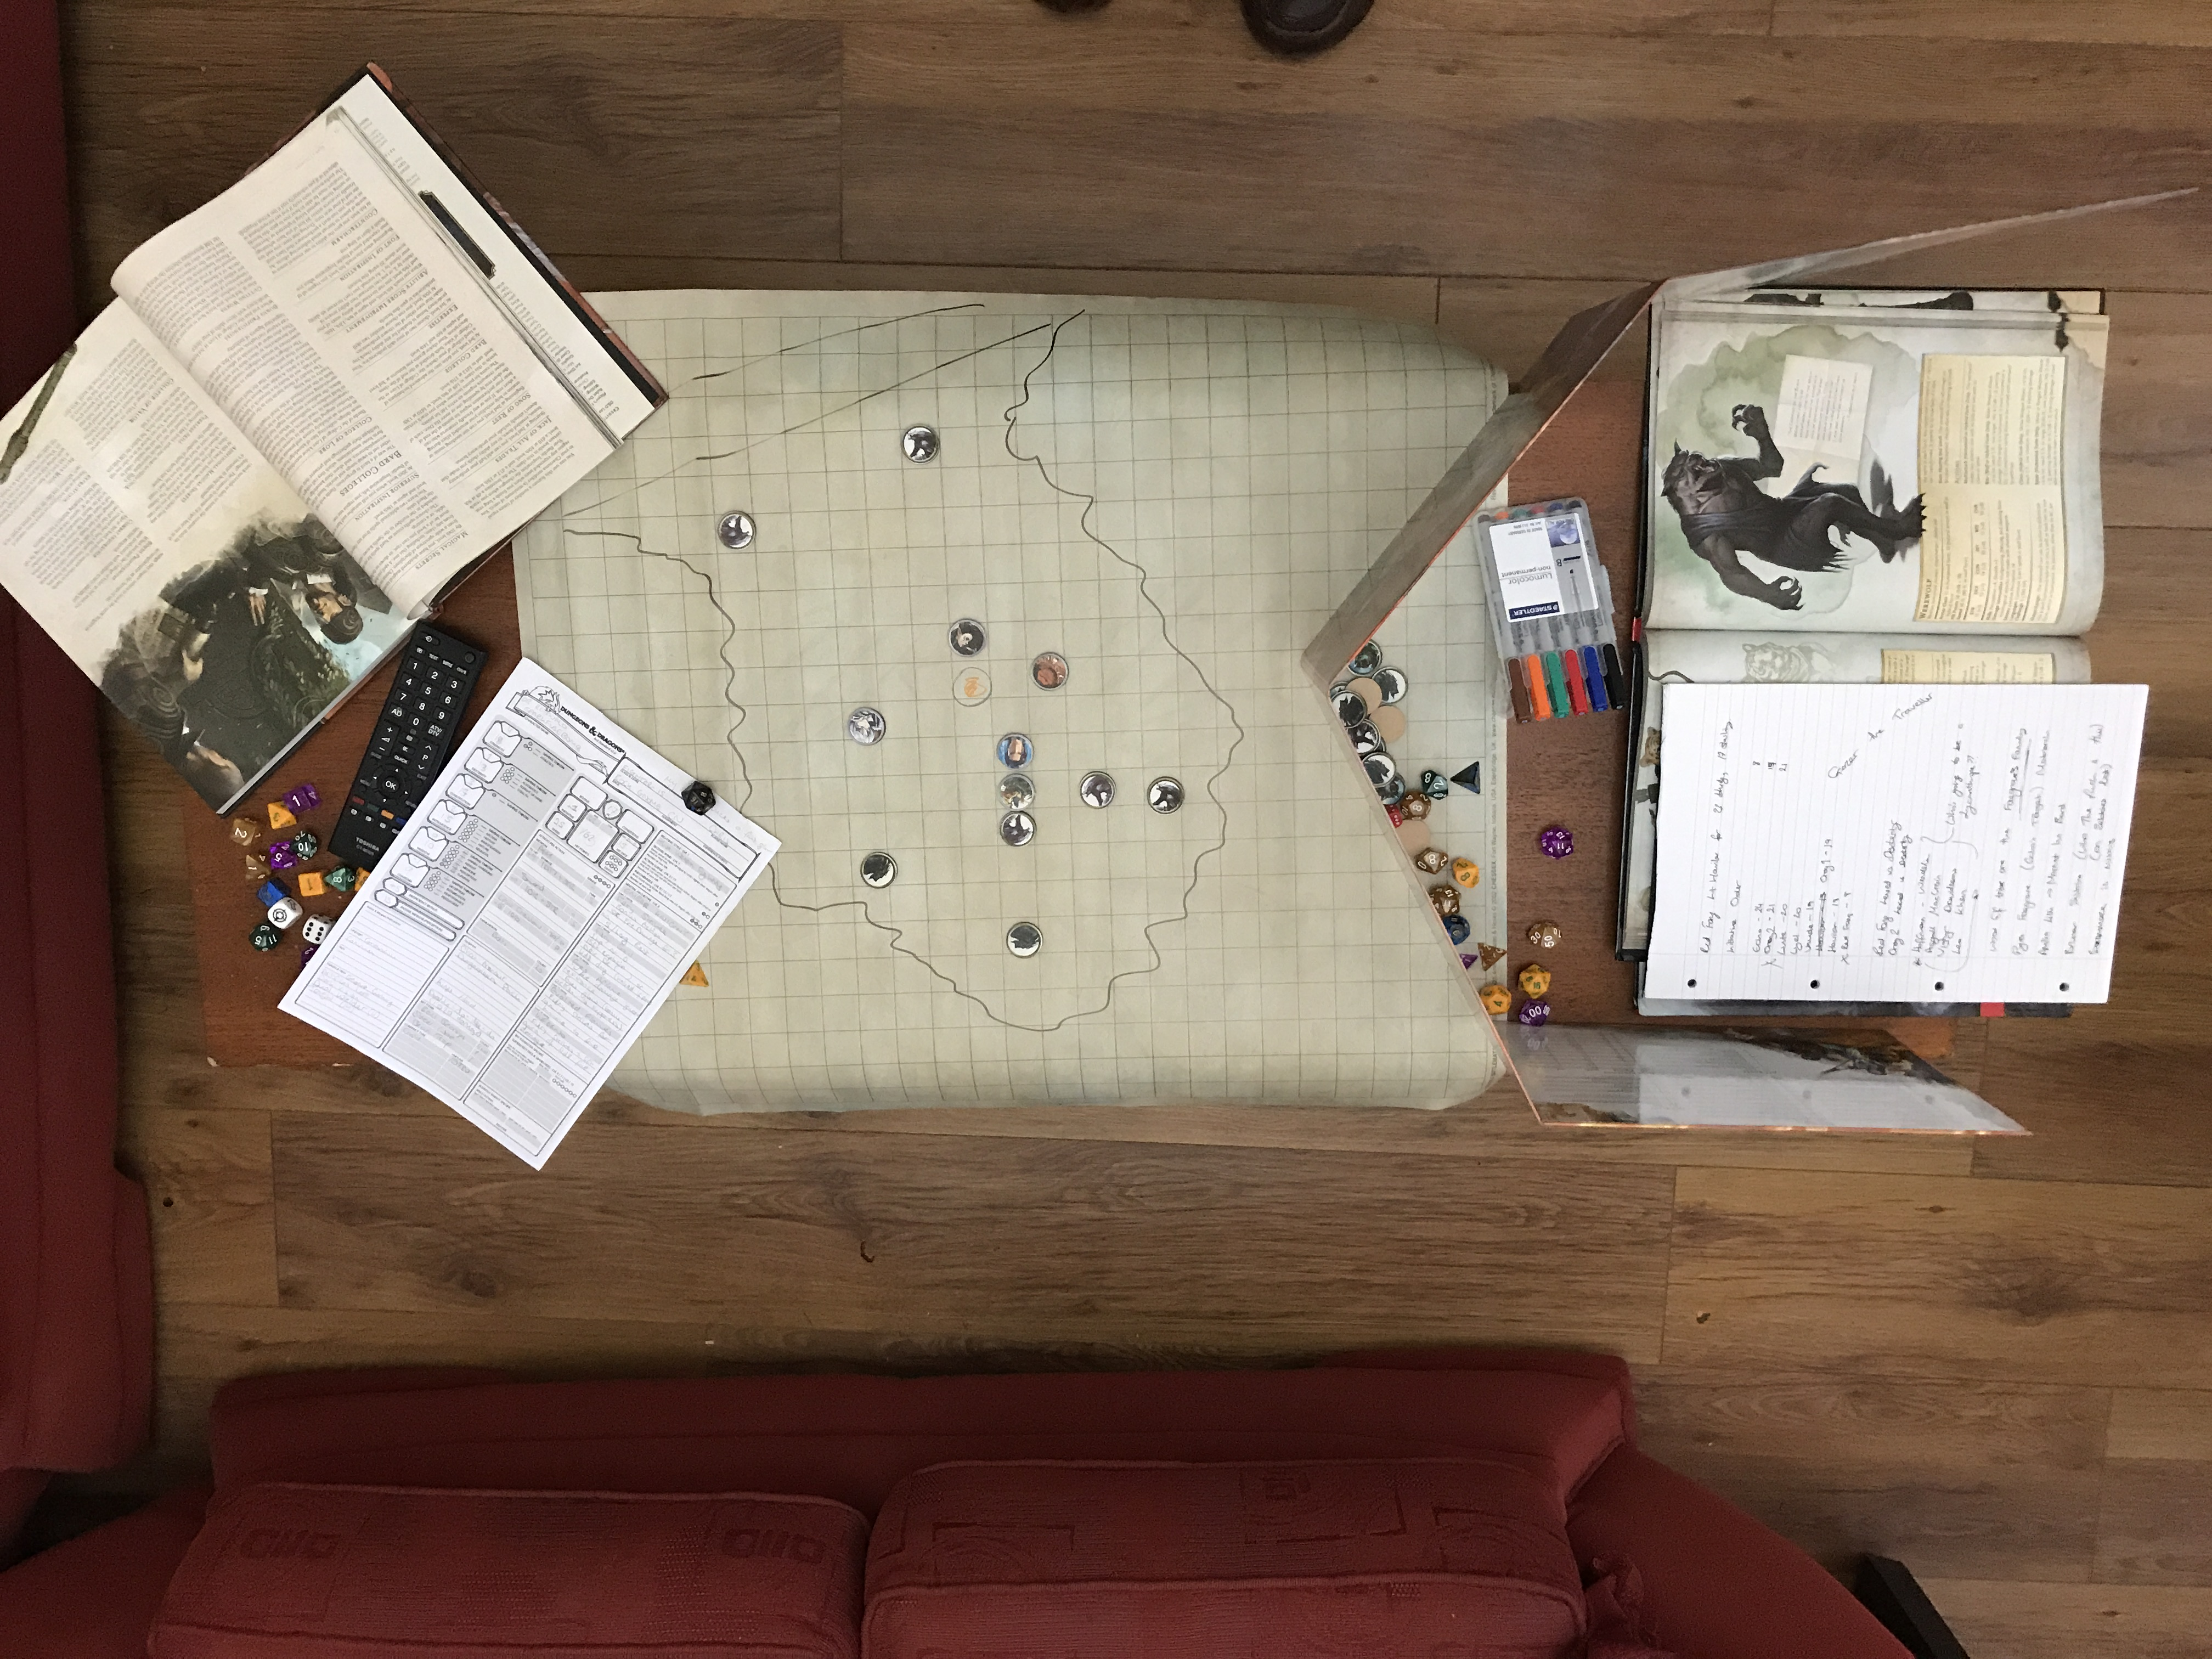
\includegraphics[width=0.9\linewidth, height=5cm, angle=180]{DnD_Live.jpg}
			\caption{A typical \dnd set up} \label{DnDLive}
		\end{subfigure}
		\begin{subfigure}{0.5\textwidth}
			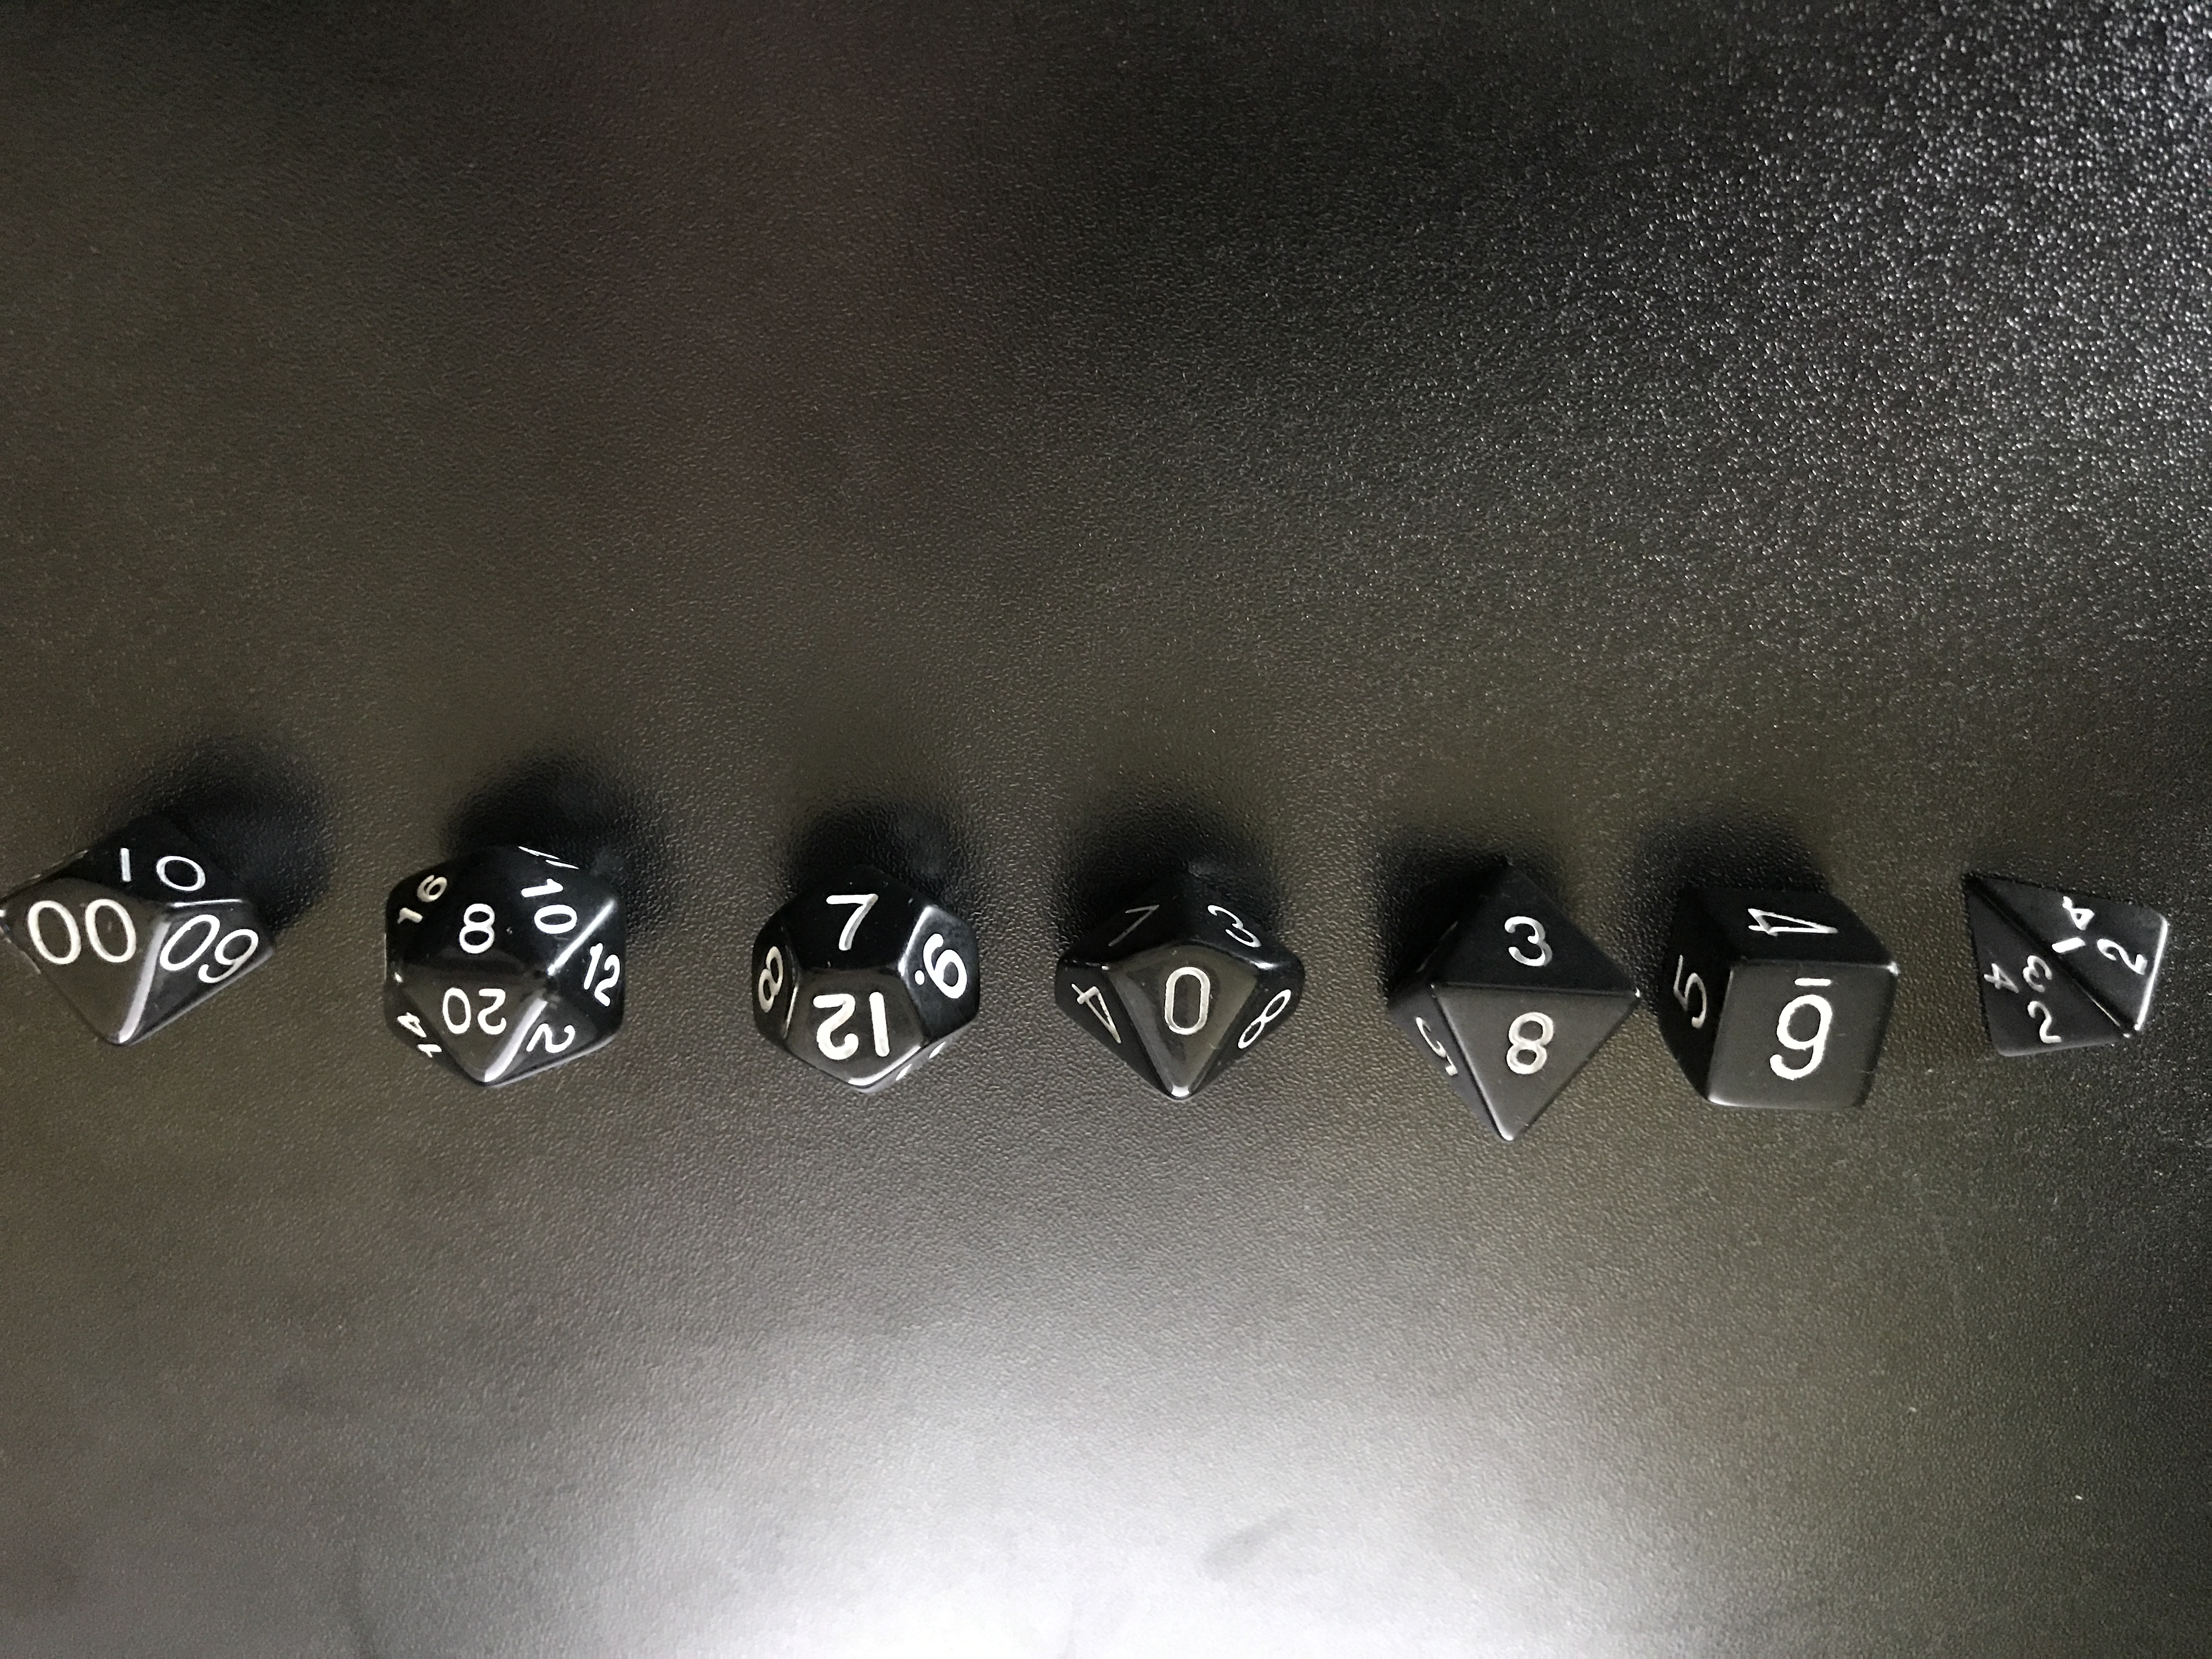
\includegraphics[width=0.9\linewidth, height=5cm, angle=180]{DnD_Dice.jpg}
			\caption{The Die necessary to play \dnd} \label{DnDDice}
		\end{subfigure}
		\caption{These two figures show the typical equipment for a \dnd \ game}
	\end{figure}

	Each group of people who play \dnd \ is divided in two, the DM and the \emph{Party}. The DM, as previously stated in the Introduction (Section \ref{intro}), runs the game and creates the content for the Party to play through. Each member in the Party controls a \emph{Player Character} (PC) for the duration of the game. The DM controls every other character, known as \emph{Non-Player Character} (NPC). The PCs and NPCs interact through \emph{encounters}, which can be friendly/hostile (see Section \ref{DnDExplore}) and may escalate to \emph{Combat} (for more details see Section \ref{DnDCombat}). In Combat, characters can affect each other with \emph{Attacks} and \emph{Spells} to either inflict \emph{Damage}, \emph{Healing} or \emph{Conditions}.
	
	As discussed in the Introduction (Section \ref{intro}), a DM will spend a portion of their time \emph{preparing content} for their game. 
	
	\Codex \ is a tool for the DM of a group to use in order that they can enjoy running games of \dnd \ to a higher degree. To do this, a limit has been set on \Codex \ scope. \Codex \ will not replace any dice rolling or the simple arithmetic that fuels the game. Instead \Codex \ will be an interface to track game statistics and quickly review rules and ability effects,  allowing the DM to instil more narrative and creative content into the game.
	
	\subsubsection{Understanding Dungeons and Dragons}
	\dnd \ is a game that is random by design, but there are two distinct areas to \dnd \, \emph{Exploration} and \emph{Combat}. \Codex \ will largely deal with the Combat rules, however there is scope to support the DMs in the Exploration area as well. There is one overarching concept about \dnd \ that needs to be understood when dealing with the rules of game. The rules are nothing more than a suggestion to the DM about how to run his or her game. Every group will have their own way of dealing with different situations, which could be an entirely new rule or an adjustment to one of the suggested rules. \dnd \ is governed by the roll of dice. The most common die that is used is the 20-sided die, which dictates if an attack hits, or if you were able to persuade a character in game. It is used in both Combat and Exploration. The other dice (100, 12, 10, 8, 6 and 4 sided) are largely used for damage or the result of a spell. These dice are denoted by a lower-case `d' and the number of side that dice possess, for example the 20-sided dice are denoted as \textbf{d20}.
	
	\subsubsection{Exploration} \label{DnDExplore}
	We shall begin with a brief look into Exploration, this is where the majority of DM preparation time is spent. DMs need to have landscapes, settlements, characters, dialogue, plot points and consequences for Players to interact with whilst they explore the world. The Dungeon Master's Guide \citep{DMGuide} contains a lot of information about the officially published settings, as well as tips and tricks for creating your own adventures. One of the most useful sources in the Dungeon Master's Guide for creating adventures for the Players to explore, is the multitude of random chance tables that allow you to create all the necessary information that forms the core of any adventure you might need for your game. These random chance tables are not limited to adventure story lines, other tables cover the characters the Players may interact with or the treasures players might receive at the end of an adventure. \Codex \ aims to include a planning feature that will integrate these tables to allow the busy DM to instantly create the framework for adventures and characters. 
	
	\subsubsection{Combat} \label{DnDCombat}
	There are a lot more combat rules than exploration rules spread throughout the three \dnd \ core books (\cite{DMGuide}, \cite{MonsterManual} and \cite{PlayerHandbook}) . These rules are also more heavily suggested towards the DM as quite often the lives of the Player's Characters depend on these rules. Some DMs do choose to alter these rules to suit their game \citep{Personal}, however \Codex \ will follow these rules as written. The Combat rules are the same for both the Player Characters and the enemies they face, and can be broken down into a set of simple calculations. For example, when seeing if an attack with a hammer will hit; the character's \emph{proficiency} \ plus \emph{strength modifier} \ will be added to the result of a \emph{d20 roll}. This can be summarised to be:

	The attack roll is 23, this is then compared against the targets \emph{Armour Class (AC)}. Plate Armour has an AC of 18, so the attack roll of 23 is greater than the AC of the target and will hit \citep{PlayerHandbook}. This rule will not be included in \Codex's scope as it is taking away enjoyment from the players and is not helping the DM do their job. Instead it is rules like the \emph{poisoned} rule that will be taken into account, where a suitable icon will be placed over the character who is \emph{poisoned}, to remind the DM that  character has the condition.
	
	\subsection{Software Engineering Models} \label{SEMLit}
	A \sem \ at its core, is a model for time management in relation to a project, particularly the Agile \sems \ \citep{AgileManifesto} - such as Scrum  \citep{Scrum} . The majority of \sems \ are focused on controlling development time and code reviews, however some can extend to managing research and design work as well. For \Codex, we will look at two potential \sems \ to support the research, design and development phases. 
	 
	\subsubsection{Agile for One}
	Agile for One is an adaptation of the Agile Manifesto to be more suitable for a single developer project, with the outcome of defining a new \sem , called Agile Solo \citep{AgileSolo}. Agile Solo is similar to traditional Scrum in that there are weekly iterations inside a longer over-arching period of time, but rather than a two-week sprint encapsulating a daily scrum meeting, there is a monthly deliverable with a weekly iteration. At the end of each week, the Developer meets with the Customer or a Supervisor to discuss what occurred during the week and what the next focus should be. A longer review takes place at the end of each month. Agile Solo also recommends a daily meeting with a fellow developer to ensure that code quality is maintained. 
	
	\subsubsection{Extreme Programming for One}
	Extreme Programming (XP) is a \sem \ which emphasises the importance of constant feedback and maintaining simplicity in a system, allowing a project to thrive in an ever-changing environment. XP For One preserves the traditional stages of XP, but the \emph{Pair Programming} recommendation is impossible to replicate in a solo developer project \citep{SoloXP}. So instead XP For One suggests; that the developer has a friend or colleague constantly check that the developer has run the tests on the current section of work, that a log book is kept detailing the tests and development results and that the developer meet with a supervisor or client regularly to maintain the constant feedback. 
	
	\subsubsection{Development of \Codex}
	The development of \Codex, which includes the non-programming activities (such as reports and presentations) will be achieved by utilising Agile for One Software Engineering Model for all aspects of the report. Trello, a website dedicated to project management, will aid in the management of tasks \citep{Trello}. Should Agile for One be unsuitable for the development of \Codex \ then Extreme Programming for One will be used.
	
	\clearpage 
	
	\subsection{Web-App Architecture} \label{Web-Arch}
	Web-App Architecture can be simplified down to three layers.
	\begin{figure}
		\centering
		\fbox{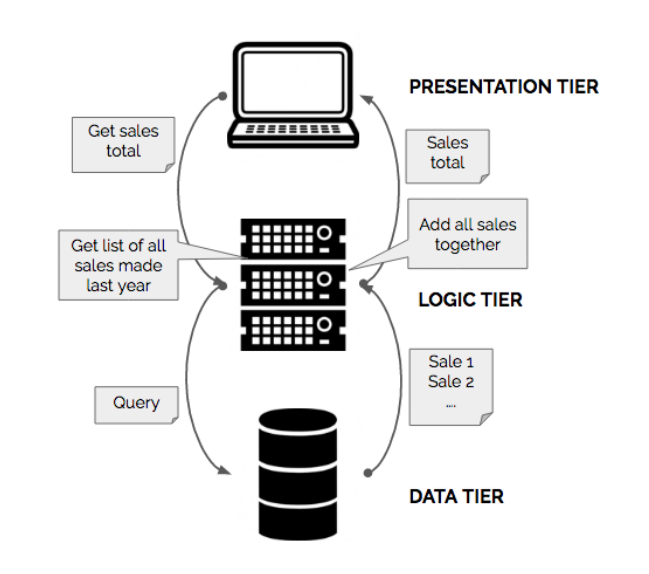
\includegraphics[width=0.5\textwidth]{Basic_Web_App_Architecture.PNG}} 
		\caption{Overview of a three-tier application and its dependencies \citep{SecurityWebApps}} \label{Web-App-Arch}
	\end{figure}
	As we can see from Figure \ref{Web-App-Arch} the first layer (Presentation Tier) is held locally on the Client's machine. This is what is known as `Client-Side'. Here HTML, CSS and JavaScript is used to translate data into a format the Client will understand. The second layer (Logic Tier), here languages such as PHP or Node.js perform functions on raw data to generate web content. Traditionally the Logic Tier is hosted on a Server that Clients connect to, this is the `Server-Side' The third layer (Data Tier) communicates with the Logic Tier through SQL Queries \citep{SecurityWebApps}.
	
	\subsubsection{Server- vs Client-Side Technologies}
	From Figure 2, we can create a rule for the division of \Codex' functions between Server- and Client-Side technologies. All data and logical functions should be hosted on the Server-Side and the display functions should be hosted on Client-Side. However, this does create a problem. This rule means that \Codex \ will have no Offline Functionality, which \Codex \ aims to have.
	
	\subsubsection{Test Driven Development (TDD) and Web-App Architecture}
	TDD is a common Software Engineering practice which dictates that when developing a function, the test for that function must be developed first so that the function can be developed to pass the test. The advantages of TDD are numerous; code is tidier, documentation is more thorough and the lower number of bugs are the main advantages towards \Codex. TDD is typically used for functional programming only therefore, it is not suited towards Web-Based languages such as HTML and CSS \citep{TDD}. But we can use TDD with PHP and JavaScript. To simplify the development of \Codex \ we will not use PHP as JavaScript can run on both the Server- and Client-Side of the app.

	\subsection{Database Design} \label{Database}
	Traditional Database Design is performed using \emph{Entity Relationship Diagrams} which tables of objects and how they are related to one-another. From there a SQL database can be built and populated on a server, ready for access \citep{DatabaseDesign}. 
	
	\subsubsection{Databases for Web-Based Internet Applications}
	The problem with this way of designing and building a database is speed. When you have a multi-tiered system, such as a Web-App (see Figure \ref{Web-App-Arch}), the access times to the database is too slow for modern users \citep{WebAppDatabase}. The solution to this issue is to have a multi-module database with the minimal amount of overhead as possible. 

	\subsection{Graphical User Interfaces} \label{GUIs}
	The GUI is, arguably, one of the most important party of any system where a user interacts directly with any part of the system. A good GUI is easy to understand and simple in its design. Ideally, every GUI should follow Norman's 8 Design Principles \citep{Norman}, but in the most systems compromises must be made. 
	
	\subsubsection{GUI Design}
	From a Software Engineering Perspective, GUI Design should come before anything else is designed. Once the system requirements have been set, \emph{low-fi} prototyping should take place for the GUI (this is usually sketched on using pen and paper). Once the \emph{low-fi} has been tested and approved, the prototypes of the GUIs become increasingly \emph{hi-fi} until you have reached an entirely digital prototype. GUI Design follows this methodology because \emph{low-fi} prototypes are cheaper and quicker to produce than \emph{hi-fi} prototypes. Once the GUI has been designed, functions and classes are created to fit the GUI \citep{GUIDesign}. 
	
	\subsubsection{GUI Testing}
	At each stage of GUI prototyping, usability testing needs to occur. This can either be a Heuristic Evaluation, with "expert users" (such as Developers, Trained Heuristic Evaluators or similar system users) or a Usability Study. In the early \emph{low-fi} stages, usually only one of these tests are applied, but as the prototype gets \emph{hi-fi} both tests are employed to provide the greatest level of feedback possible \citep{GUIDesign}.
	
	\subsubsection{Mobile GUI Design and Testing}
	Mobile GUIs have been around for a while, ever since the rise of the smart phone in late 00's. At first Mobile Apps and Websites had to be separate, dedicated entities \citep{MobileUsability}. There have been advances in Web-Technologies since then allowing for the same service to scale down to a smaller screen side. 
	
	\clearpage
	
	\appendix
	
	\section{\Codex \ Gantt Chart}
	\begin{cmpfigure}{\Codex \ Gantt Chart, outlining the major tasks and deliverables\label{pplan}}
		\begin{sideways}
			\newganttchartelement{voidbar}{
				voidbar/.style={draw=black, top color=black!25, bottom color=black!23
			}}
			\begin{ganttchart}[y unit chart = 0.86cm, y unit title = 0.86cm, x unit=0.45cm, vgrid, title label font=\scriptsize,
				canvas/.style={draw=black, dotted}]{1}{34}
				\gantttitle{Project schedule shown for e-vision week numbers
					and semester week numbers}{34} \\
				
				\gantttitlelist{8,...,41}{1}\\
				\gantttitlelist{1,...,12}{1} \gantttitle{CB}{4}
				\gantttitlelist{1,...,9}{1} \gantttitle{EB}{4}
				\gantttitlelist{10,...,14}{1}\\
				
				%The elements, bars and milestones, are identified as elem0, elem1, etc.
				\ganttbar{Project Proposal}{1}{2} \\        		%elem0  
				\ganttbar{Literature Review}{2}{5} \\      			%elem1 
				\ganttmilestone{Literature Review Finished}{5} \\	%elem2
				\ganttbar{Design Doc. Iteration 1}{4}{8} \\ 		%elem3
				\ganttbar{Development Iteration 1}{9}{11} \\		%elem4
				\ganttbar{Progress Report}{11}{12} 					%elem5
				\ganttmilestone{}{12} \\							%elem6
				\ganttbar{Development Iteration 2}{11}{12}  		%elem7
				%week 1 of semester 2 is the 17th week in schedule 
				\ganttvoidbar{}{13}{16} \\                     		%elem8
				\ganttbar{Final Report Writing 1}{17}{19} 	        %elem9
				\ganttmilestone{}{19} \\							%elem10
				\ganttbar{Design Doc. Iteration 2}{19}{20} \\      	%elem11
				\ganttbar{Development Iteration 3}{21}{26} \\		%elem12
				\ganttbar{Testing}{24}{26} \\						%elem13
				\ganttmilestone{Code Delivery}{26} \\       		%elem14
				\ganttbar{Final Report Writing 2}{27}{30} \\  		%elem15
				\ganttbar{Inspection preparation}{31}{34}   		%elem16
				
				\ganttlink{elem0}{elem1} \ganttlink{elem1}{elem2} \ganttlink{elem2}{elem3}
				\ganttlink{elem3}{elem4} \ganttlink{elem4}{elem5} \ganttlink{elem5}{elem6}
				\ganttlink{elem5}{elem7} \ganttlink{elem8}{elem9} \ganttlink{elem10}{elem11}
				\ganttlink{elem11}{elem12} \ganttlink{elem12}{elem13} 
				\ganttlink{elem13}{elem14} \ganttlink{elem14}{elem15}
				\ganttlink{elem15}{elem16}
			\end{ganttchart}
		\end{sideways}
	\end{cmpfigure}

	\clearpage
	
	
	\clearpage	
\bibliography{projectbib}
\end{document}
% EOF Document